\section{Multiple Domain Experiments}
\label{sec:multi_domain}


In order to test whether our findings and scaling law formula extend to settings with more than one constrained domain, we set up experiments with a mixture of three domains: one unconstrained generic source and two constrained target domains.
We use two configurations: FineWeb as the generic source with peS2o and Wikipedia as targets, and Nemotron as the generic source with Wikipedia and peS2o as targets.\footnote{Subplot~(a) of Figure~\ref{fig:3domain_combined} uses FineWeb + peS2o + Wikipedia; subplots~(b) and~(c) use Nemotron + Wikipedia + peS2o.}
We vary the dataset sizes across three configurations: 5$\times$ less, base, and 5$\times$ more data.
Our primary metric is the average loss across both target domains, analogous to evaluating on a test set that combines text from both domains.


\begin{figure*}[t]
   \centering
   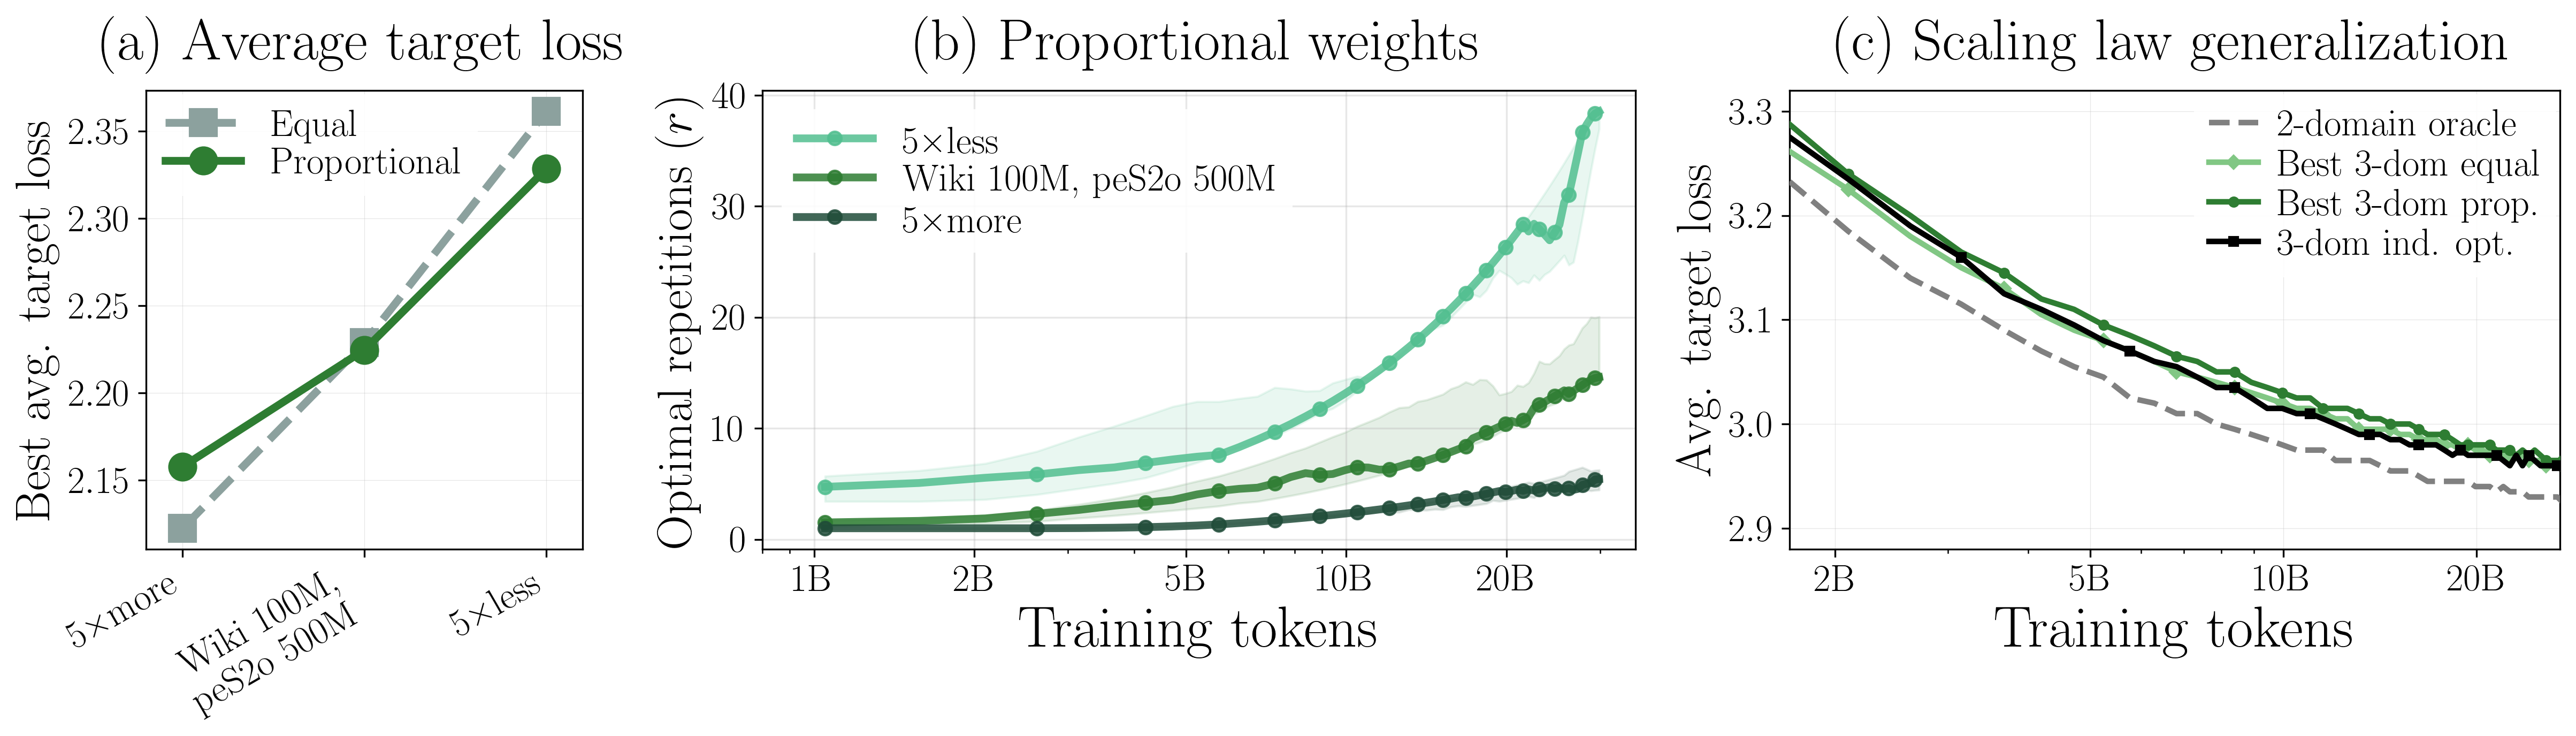
\includegraphics[width=\textwidth]{figures/fig_3domain_combined_3panel.png}
   \vspace{-15pt}
   \caption{Multi-domain experiments (101M model, English + Wikipedia + peS2o). \textbf{(a)} Best achievable average target loss under equal vs.\ proportional weighting across three set-size configurations. \textbf{(b)} Optimal repetitions under proportional weighting with 10\% compute confidence band (shaded). \textbf{(c)} Independently optimizing $r$ per domain using the bilingual scaling law outperforms the best grid-searched proportional weighting.}
   \vspace{-10pt}
   \label{fig:3domain_combined}
\end{figure*}

\paragraph{Weighting Strategies}
First, we compared two weighting strategies: \emph{equal weighting} ($h_{\text{wiki}} = h_{\text{peS2o}}$) and \emph{proportional weighting}, where fractions are set proportional to dataset size ($h_{\text{wiki}} / h_{\text{peS2o}} = D_{\text{wiki}} / D_{\text{peS2o}}$).
Our experiments demonstrate (Figure~\ref{fig:3domain_combined}a) that by average loss, proportional weighting outperforms equal weighting when data is scarce, while equal weighting is better in the data-rich regime. 
The two strategies cross near the base configuration, suggesting that proportional weighting becomes increasingly beneficial as repetition grows. 
For the rest of this section, we focus on the proportional weighting, and provide the results for equal weighting in Appendix~\ref{app:3domain}. 

\paragraph{Empirical Findings}
The key findings from the bilingual experiments carry over to the multi-domain setting.
Figure~\ref{fig:3domain_combined}b shows that optimal repetition grows steadily with training tokens across all set-size configurations, with smaller sets requiring substantially higher repetition: the 5$\times$less variant reaches $r \approx 30$ while 5$\times$more stays below $r \approx 7$. This mirrors the bilingual experiments: the generic domain continues to regularize training even with multiple constrained domains present, enabling high repetition tolerance. 
Importantly, the choice of $r$ need not be exact. We quantify this through a 10\% compute confidence band (shaded regions in Figure~\ref{fig:3domain_combined}b): at each checkpoint, we identify all values of $r$ that achieve loss no worse than the best loss achievable with 10\% less compute. The bands are wide, particularly for smaller sets, indicating that even rough estimates of optimal $r$ yield near-optimal target loss.



\paragraph{Scaling Law Generalization}
The similarity of these findings to the bilingual setting raises the question of whether the scaling law transfers directly to multi-domain mixtures. We test this by setting each domain's repetition factor independently using the optimal $r$ predicted by the bilingual scaling law for the corresponding set size ($r_\text{wiki}=35$, $r_\text{peS2o}=17$). Figure~\ref{fig:3domain_combined}c shows that this independently optimized configuration consistently outperforms the best proportional weighting and narrows the gap to the 2-domain oracle (the average loss achieved by training each domain separately with English). While a gap to the oracle remains, this result suggests that costly multi-domain sweeps over all possible combinations of domain weights can be avoided: our two-domain scaling law can independently estimate the optimal $r$ for each constrained domain, and these can be combined into a single mixture, replacing an entire experimental grid with a single, better-performing run.

